\documentclass[11pt,a4paper,DIV=12]{scrartcl}	
\usepackage[T1]{fontenc}
\usepackage[utf8]{inputenc}
\usepackage[ngerman]{babel}	
\usepackage{xcolor}		
\usepackage{graphicx}
\usepackage{tabularx}
\usepackage{textcomp,paralist}
\usepackage{booktabs,array,longtable}
\usepackage{libertine}

\begin{document}

\definecolor{BlauTierraNueva}{cmyk}{0.75, 0.38, 0, 0.45}

\parindent0mm
\renewcommand{\arraystretch}{1.2}

\newenvironment{literatur}{%
  \parskip6pt \parindent0pt \raggedright
  \def\lititem{\hangindent=0.3cm \hangafter1}}{%
  \par\ignorespaces} 

\begin{figure}
\begin{minipage}{0.6\linewidth}
{\Huge \textsc{\textcolor{BlauTierraNueva}{Curriculum Vitae}}}\\[0.7cm]
{\Large \textsc{Tiberius Tölpel}}\\[0.2cm]
Hermannweg 3\\
D-01234 Bellinghausen\\
+49-(0)123\,66\,28\,43\,00\\
ttölpel@vogelmann.com\\[-1.5cm]
\end{minipage}
\begin{minipage}{0.4\linewidth}
\hspace*{2.2cm} 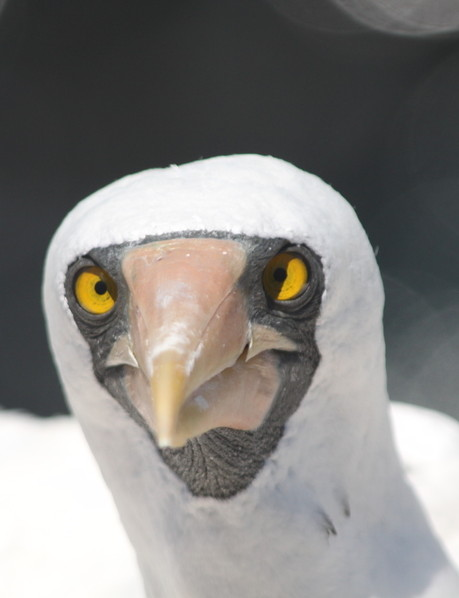
\includegraphics[width=0.6\textwidth]{Passbild.jpg}
\end{minipage}
\end{figure}

\vspace*{0.3cm}

\begin{tabularx}{\textwidth}{p{2.8cm}X}
Geboren am: & 01. Januar 1977, Tölpelhausen, Deutschland\\
\end{tabularx}

\vspace*{0.9cm}

\textsc{Ausbildung und wissenschaftlicher Werdegang}\par
\noindent\rule[1ex]{\textwidth}{0.2pt}

\begin{longtable}{>{\raggedright \arraybackslash}p{2.8cm}
>{\raggedright \arraybackslash}p{11.5cm}}
02/2009--01/2014 	& 	\textbf{Wissenschaftlicher Mitarbeiter}, Universität Tölpelstedt
	\linebreak inkl. \textbf{Promotion}: »Neue Erkenntnisse aus der Erforschung von Tölpelfedern«, Betreuer: Prof. G. Schwalbe (Uni Schwalbhausen)\\
	
06/2010 & \textbf{Diplom-Abschluss} als Diplom-Vogelkundler, Uni Bechterstedt
	\linebreak \hspace*{0.7cm} Note: \textbf{1,2} (sehr gut)\\
	
2008/2009 & 	\textbf{Diplomarbeit}: »Wege zur Erbeutung von Futter aus Menschenhand«, Betreuer: Prof. R.\,R. Rabe (Uni Nesterstedt)
	\linebreak \hspace*{0.7cm} Note: \textbf{1,4} (sehr gut)\\
	
2010	 & \textbf{Mündliche Prüfungen}
	\linebreak \hspace*{0.7cm} Geschrei/Aufmerksamkeit: \textbf{1,0} (sehr gut)
	\linebreak \hspace*{0.7cm} Nestbau/Hege: \textbf{1,7} (gut)
	\linebreak \hspace*{0.7cm} Futtersuche/Gefahren: \textbf{2,0} (gut)
	\linebreak \hspace*{0.7cm} Flugmanöver: \textbf{1,7} (gut)\\
	
01/1990--08/1993 	& 	\textbf{Vogelschule}, Ringenstedt\\
\end{longtable}

\vspace*{0.3cm}

%%%%%%%%%%%%%%%%%%%%%%%%%%%%%%%%%%%%%%%%%%%%%%%%%%%%%%%%%%%%%%%%%%%%%%%%%%%%%

\textsc{Auslandserfahrung}\par
\noindent\rule[1ex]{\textwidth}{0.2pt}

\begin{longtable}{>{\raggedright \arraybackslash}p{2.8cm}
>{\raggedright \arraybackslash}p{11.5cm}}
07--09/2009 		& 	\textbf{Überflug Nordskandinaviens}	
	\linebreak {\small \textit{Beobachtung und Erfassung geeigneter Nistplätze}}\\
01--02/2006 		& 	\textbf{Erkundung von W-Europa}, Spanien
	\linebreak {\small \textit{Suche nach Fortpflanzungspartner}, Leitung: Dr. F. Krauskopf}\\
\end{longtable}
\vspace*{0.3cm}

%%%%%%%%%%%%%%%%%%%%%%%%%%%%%%%%%%%%%%%%%%%%%%%%%%%%%%%%%%%%%%%%%%%%%%%%%%%%%

\textsc{Zusätzliche Erfahrung}\par
\noindent\rule[1ex]{\textwidth}{0.2pt}

\begin{longtable}{>{\raggedright \arraybackslash}p{2.8cm}
>{\raggedright \arraybackslash}p{11.5cm}}
03/2009--04/2010		& \textbf{Fortbildung}, Uni Hammach
	\linebreak	{\small \textit{Gefiederpflege und -schmuck}}\\
\end{longtable}
\vspace*{0.3cm}

%%%%%%%%%%%%%%%%%%%%%%%%%%%%%%%%%%%%%%%%%%%%%%%%%%%%%%%%%%%%%%%%%%%%%%%%%%%%%
\newpage
\textsc{Wissenschaftliche Veröffentlichungen}\par
\noindent\rule[1ex]{\textwidth}{0.2pt}

\begin{literatur}

\lititem \textsc{Tölpel,~T.}, \textsc{Spatz,~G.} \& \textsc{Adler,~A.} (2014): Über die Rundung von Eiern. -- Vogelzeitschrift, 223(3): 23--44.

\lititem \textsc{Tölpel,~T.} \& \textsc{Geier, V.} (2006): Was man vom Überwintern lernen kann: Möglichkeiten und Alternativen zum Federwechsel. -- Journal for Ornithology, 44(2): 1--77.
		
\end{literatur}

\vspace*{0.8cm}

%%%%%%%%%%%%%%%%%%%%%%%%%%%%%%%%%%%%%%%%%%%%%%%%%%%%%%%%%%%%%%%%%%%%%%%%%%%%%

\textsc{Öffentliche Vorträge und Poster}\par
\noindent\rule[1ex]{\textwidth}{0.2pt}

\begin{longtable}{>{\raggedright \arraybackslash}p{2.8cm}
>{\raggedright \arraybackslash}p{11.5cm}}
02/2005 & 	\textbf{Vortrag:} »Eingangsrede zur Eröffnung des neuen Vogelbauers im Dorf«
		\linebreak {\small \textit{Vogeltagung 2005, Ufterhausen}}\\
		
09/2002	& \textbf{Poster:} »Die Kunst der Entblößung: Geheime Botschaften in Vogelkot«
	\linebreak {\small\textit{Tagung für Vogelfreunde, Rungelhausen}}\\

\end{longtable}

\vspace*{0.3cm}

%%%%%%%%%%%%%%%%%%%%%%%%%%%%%%%%%%%%%%%%%%%%%%%%%%%%%%%%%%%%%%%%%%%%%%%%%%%%%
\textsc{Teilnahme an Tagungen und Workshops}\par
\noindent\rule[1ex]{\textwidth}{0.2pt}

\begin{longtable}{>{\raggedright \arraybackslash}p{2.8cm}
>{\raggedright \arraybackslash}p{11.5cm}}

01/2004 & 	\textbf{Ornithologic Workshop 2004}
	\linebreak {\small\textit{Nist- und Brutplätze artverwandter Tölpel in Süd-England}, Leitung: Dr. E.~Meise (London)}\\

\end{longtable}
\vspace*{0.3cm}

%%%%%%%%%%%%%%%%%%%%%%%%%%%%%%%%%%%%%%%%%%%%%%%%%%%%%%%%%%%%%%%%%%%%%%%%%%%%%

\textsc{Mitgliedschaften}\par
\noindent\rule[1ex]{\textwidth}{0.2pt}

\begin{longtable}{>{\raggedright \arraybackslash}p{2.8cm}
>{\raggedright \arraybackslash}p{11.5cm}}
	seit 2011 & Mitglied der Tölpel-Subkommission\\
\end{longtable}
\vspace*{0.3cm}

%%%%%%%%%%%%%%%%%%%%%%%%%%%%%%%%%%%%%%%%%%%%%%%%%%%%%%%%%%%%%%%%%%%%%%%%%%%%%

\textsc{Sprachkenntnisse}\par
\noindent\rule[1ex]{\textwidth}{0.2pt}

\begin{longtable}{>{\raggedright \arraybackslash}p{2.8cm}
>{\raggedright \arraybackslash}p{11.5cm}}
	Tölpelisch & Muttersprache\\
	Geierisch & flüssig\\
\end{longtable}
\vspace*{0.3cm}

%%%%%%%%%%%%%%%%%%%%%%%%%%%%%%%%%%%%%%%%%%%%%%%%%%%%%%%%%%%%%%%%%%%%%%%%%%%%%

\textsc{EDV-Kenntnisse}\par
\noindent\rule[1ex]{\textwidth}{0.2pt}

\begin{longtable}{>{\raggedright \arraybackslash}p{2.8cm}
>{\raggedright \arraybackslash}p{11.5cm}}
Betriebssysteme		& 	WingOS, Linux\\
Büro-Software 		& 	BirdyOffice\\
Grafik-Software 	& 	PhotoTölp 3.2\\
\end{longtable}
\vspace*{0.3cm}

%%%%%%%%%%%%%%%%%%%%%%%%%%%%%%%%%%%%%%%%%%%%%%%%%%%%%%%%%%%%%%%%%%%%%%%%%%%%%
\newpage
\textsc{Führerschein}\par
\noindent\rule[1ex]{\textwidth}{0.2pt}

\begin{longtable}{>{\raggedright \arraybackslash}p{2.8cm}
>{\raggedright \arraybackslash}p{11.5cm}}
Klasse B & eigener PKW\\
\end{longtable}
\vspace*{0.3cm}

%%%%%%%%%%%%%%%%%%%%%%%%%%%%%%%%%%%%%%%%%%%%%%%%%%%%%%%%%%%%%%%%%%%%%%%%%%%%%
\textsc{Interessen und Hobbys}\par
\noindent\rule[1ex]{\textwidth}{0.2pt}

\begin{compactitem}
	\item Fische fangen, Dösen
	\item Müll fressen, Ausflüge über Land
\end{compactitem}
\vspace*{3cm}

Dinkelhausen, \today

\end{document}
